\resetfigpath{Intro}

%%%%%%%%%%%%%%%%%%%%%%%%%%%%
%{SUMMARY FOR ALL CHAPTERS}%
%%%%%%%%%%%%%%%%%%%%%%%%%%%%

Complex interactions between drivers are often observed at urban crossroads, especially those without traffic signals. In this thesis, the human driver behaviors at crossroads are modeled in a probabilistic way. In the Chapter~\ref{chap:Lit}, techniques for motion planning are reviewed. Similar topics regarding the behavior prediction at the crossroad are also brought out. The central idea of this thesis is introduced in Chapter~\ref{chap:DriverModel}, where the cognitive states during the interaction are examined and modeled. The parameters representing the driving styles of drivers are attempted to identify in Chapter~\ref{chap:ModelParam}. In Chapter~\ref{chap:App}, possible applications of the proposed model are explored and verified. Finally, the conclusions and future works are discussed and listed in Chapter~\ref{chap:ConcluNFuture}. 

%%%%%%%%%%%%%%
%{Motivation}%
%%%%%%%%%%%%%%
\section{Motivation}

Since 2006, the year when the concept of autonomous vehicles came alive and into urban environments, the autonomous vehicle industry has been growing rapidly \cite{thrun2006}. Before the end of 2018, Waymo's self-driving vehicles had driven more than 10 million miles in 25 cities across the United States. Besides Waymo, 47 autonomous vehicle companies are also testing their self-driving cars in the urban area of California. Those optimistic predictions claim that by 2030, most of the human driving vehicles will be replaced by autonomous vehicles, and that it will be a solution to congestion, accidents due to human errors and air pollution. However, it doesn't seem to be so simple. 

First, according to the work of Bansal et al. \cite{Prateek2017}, fully autonomous vehicles are unlikely to be ready by 2030. They also use a simulation-based fleet evolution framework to predict long-term (year 2015-2045) adoption rates of connected and autonomous vehicles (CAVs) under different scenarios. The result suggests that the vehicle fleet is likely to have only 24.8\% level 4 (which is level 5 using the current definition of US Department of Transportation \cite{AV_levels2019}) autonomous vehicle penetration by 2045. McKinsey \& Company and Frost and Sullivan also forecast that only 15\% of passenger vehicles will be fully autonomous by 2030 and that level 3 and level 4 are expected to account for approximately 0.8\% and 2.3\% by 2023. 

Apart from the fact that the technology itself is still at a preliminary stage where there is no commercially available level 4 vehicles exist in the market. The amount of autonomous vehicles needs to reach a certain threshold for more practical discussions, such as policy, legislation, infrastructure and consumer acceptance \cite{litman2015}. Before these four key components and the technology itself are well prepared, it is not possible to see fully autonomous vehicle being adopted by 100\%. As a consequence, it is foreseeable that the human-driving and computer-driving \textit{mixed traffic flow} will comprises the major part of the traffic flow during the transition stage that might last more than 30 years. Therefore, the major challenge during this stage would be the interaction between human drivers and computer drivers.

\begin{figure}[htbp]
\begin{center}
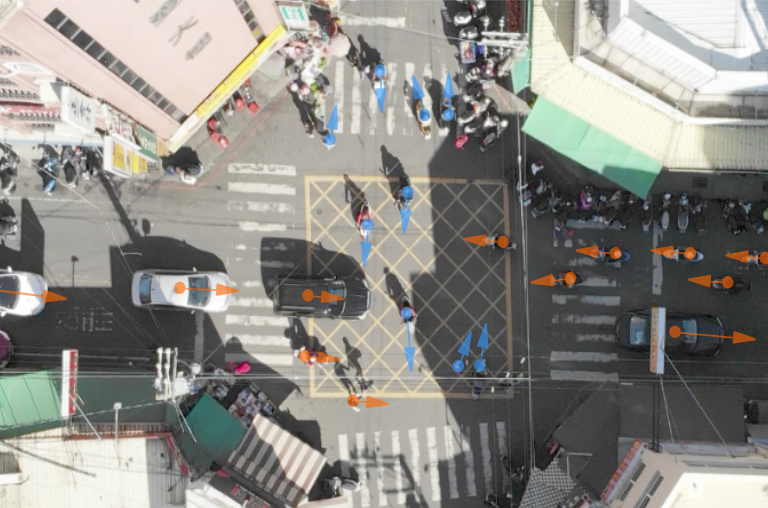
\includegraphics[scale=0.5]{complex_intersection_mod_demo.png}
\end{center}
\caption{A crossroad with no signal.}
\label{INTERSECTION} 
\end{figure}

In most of urban traffic scenarios, such as merging into lanes, entering roundabouts and crossing over crossroads without signals, drivers rely heavily on interactions with surrounding agents to blend in the traffic. For example, in Fig.~\ref{INTERSECTION} an unsignalized crossroad in central Taiwan is shown. Colored arrows represent the velocity vectors of the traffic participants. In the scene, interactions among traffic participants are based on their perception of others' intentions, and their capability in presenting their own. For example, at an unsignalized intersection, human drivers usually slow down (but not entirely stopped) or do some gesture if they intend to yield. Autonomous vehicles, on the other hand, might pose a threat to road traffic safety due to the lack of the ability to perceive the intentions of surrounding agents. According to the report of traffic collision involving autonomous vehicles published by the state of California Department of Motor Vehicles (DMV) \cite{CADMV}, autonomous vehicles being rear-ended accounts for 18 of the 33 filed reports in 2019 (as of June 17, 2019). Even though there is not much detailed documentation describing how the accident happened, we still can learn the fact that most of the accidents (over 60\%) happened while the autonomous vehicle was yielding to someone. Autonomous vehicles are designed to drive conservatively for the cause of safety, but when those behaviours are not understandable to human drivers, autonomous vehicles become a potential threats to other road users.

This research presents and initial attempt to comprehend the intentions of human drivers at an unsignalized intersection, where drivers, no matter humans or computers, are required to have more intense interaction than those at other intersections with signals or explicit rules. The targeted driver behavior model should enable the computer driver to understand and interact with human drivers smoothly so as to eliminate the potential threats in human-computer mixed traffic flow. Primary goals as well as the process of the model construction are listed as follow:

\begin{enumerate}

    \item \textbf{Driver decision making process} \\
        How human drivers perceive and react to the traffic participants at the crossroad is required to be identified.
    \item \textbf{Driver behaviors modeling in a probabilistic way}\\
        Based on the current states of the target driver, a probabilistic model that accounts for the behaviors is needed.
    \item \textbf{Driver parameters identification}\\
        Characteristic parameters representing the driving styles of the driver should be defined.
    \item \textbf{Procedure for complex interaction}\\
        Based on the proposed model, a procedure should be defined for autonomous vehicle to handle complex interaction with human drivers.

\end{enumerate}


\section{Thesis Structure}
The structure of this thesis and the objectives of each chapter is listed below (as shown in Fig.~\ref{thesis_struct}).
\begin{itemize}
    \item Chapter I : Introduction\\
        The motivation and the objectives of this thesis are introduced.
    \item Chapter II : Background and Literature Review\\
        Researches regarding the driver behaviors are reviewed.
    \item Chapter III : Human Driver Modeling at Crossroads\\
        A probabilistic driver behaviors model is proposed and verified.
    \item Chapter IV : Model Parameters Identification\\
        Parameters representing driving styles are discussed and attempted to identify.
    \item Chapter V : Applications\\
        Possible application based on the proposed model are explored.
    \item Chapter VI : Conclusions and Future Works\\
        Conclusions of this thesis and future research directions are delivered.
\end{itemize}



\begin{figure}[htbp]
\begin{center}
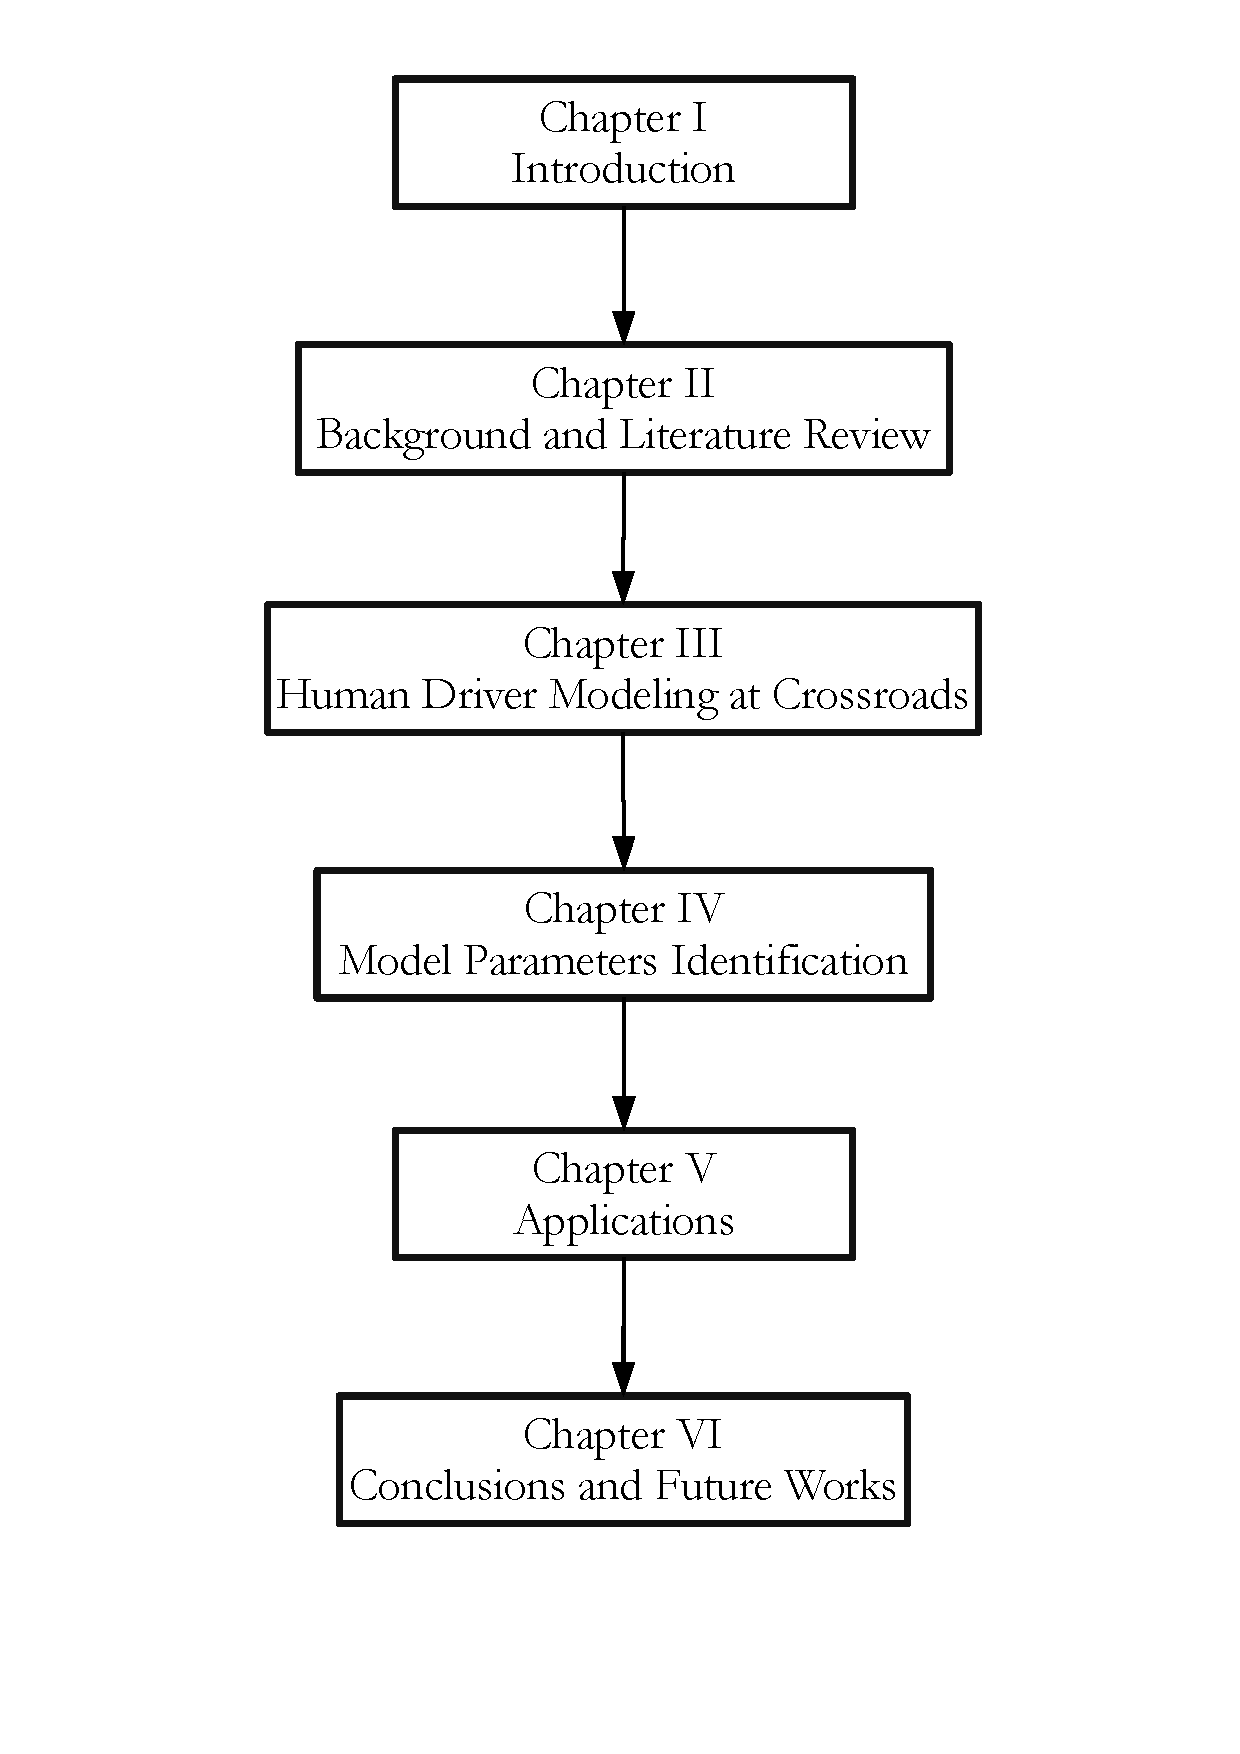
\includegraphics[scale=0.44]{thesis_structure.pdf}
\end{center}
\caption{Thesis structure.}
\label{thesis_struct} 
\end{figure}